\documentclass[12pt]{article}
\usepackage{tikz}
\usepackage{collcell}
\usepackage{xcolor}
\usepackage{pgf}

% Define the minimum and maximum values for gradient coloring
\newcommand*{\MinValue}{0}%
\newcommand*{\MaxValue}{1}%

% Apply gradient coloring based on the value
\newcommand{\ApplyGradient}[1]{%
    \pgfmathsetmacro{\PercentColor}{(#1-\MinValue)/(\MaxValue-\MinValue)*100}
    \hspace{-0.33em}\colorbox{white!\PercentColor!blue}{\textcolor{black}{#1}}
}

\newcolumntype{R}{>{\collectcell\ApplyGradient}c<{\endcollectcell}}
\renewcommand{\arraystretch}{0}
\setlength{\fboxsep}{3mm} % box size
\setlength{\tabcolsep}{0pt}

% PCA reconstructed Iself Time Domain %

\begin{document}
\begin{table}[ht]
\centering
\caption{PCA reconstructed Iself Time Domain}
\vspace{10pt} % Add more space here
\begin{tabular}{c *{5}{R}}
\multicolumn{1}{c}{} & \multicolumn{1}{c}{Matched} & \multicolumn{1}{c}{One-Head} & \multicolumn{1}{c}{One-Data} & \multicolumn{1}{c}{Random} & \multicolumn{1}{c}{Sensor} \\
Pearson's & 0.9923 & 0.9556 & 0.9949 & 0.9920 & 0.9360\\
\end{tabular}

% Color Scale
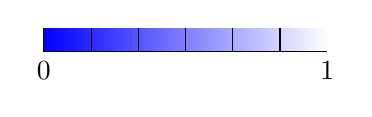
\begin{tikzpicture}[scale=0.6]
    \fill[left color=blue, right color=white] (0,0) rectangle (6,0.5);
    \draw (0,0) -- (6,0);
    \foreach \x in {0,20,...,100}
        \draw ({\x/20},0) -- ({\x/20},0.5);
    \node[below] at (0,0) {\MinValue};
    \node[below] at (6,0) {\MaxValue};
\end{tikzpicture}
\end{table}


% PCA reconstructed Iself delta frequency %
\begin{table}[ht]
\centering
\caption{PCA reconstructed Iself delta frequency}
\vspace{10pt} % Add more space here
\begin{tabular}{c *{5}{R}}
\multicolumn{1}{c}{} & \multicolumn{1}{c}{Matched} & \multicolumn{1}{c}{One-Head} & \multicolumn{1}{c}{One-Data} & \multicolumn{1}{c}{Random} & \multicolumn{1}{c}{Sensor} \\
AECno ort & 0.9718 & 0.4146 & 0.9840 & 0.9711 & 0.4207 \\
AECort &  0.8057 & 0.2264 & 0.8080 & 0.8194 & 0.3051\\
ciPLV & 0.8624 & 0.8501 & 0.7776 & 0.8499 & 0.8293\\
\end{tabular}

% Color Scale
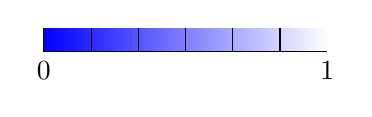
\begin{tikzpicture}[scale=0.6]
    \fill[left color=blue, right color=white] (0,0) rectangle (6,0.5);
    \draw (0,0) -- (6,0);
    \foreach \x in {0,20,...,100}
        \draw ({\x/20},0) -- ({\x/20},0.5);
    \node[below] at (0,0) {\MinValue};
    \node[below] at (6,0) {\MaxValue};
\end{tikzpicture}
\end{table}

% PCA reconstructed Iself theta frequency %

\begin{table}[ht]
\centering
\caption{PCA reconstructed Iself theta frequency}
\vspace{10pt} % Add more space here
\begin{tabular}{c *{5}{R}}
\multicolumn{1}{c}{} & \multicolumn{1}{c}{Matched} & \multicolumn{1}{c}{One-Head} & \multicolumn{1}{c}{One-Data} & \multicolumn{1}{c}{Random} & \multicolumn{1}{c}{Sensor} \\
AECno ort & 0.9764 & 0.4988 & 0.9915 & 0.9751 & 0.6357\\
AECort & 0.8558 & 0.3053 & 0.9368 & 0.8456 & 0.4749\\
ciPLV &  0.8733 & 0.8599 & 0.8939 & 0.8778 & 0.8728\\
\end{tabular}

% Color Scale
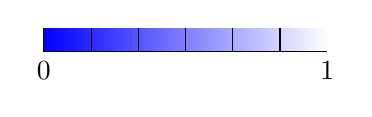
\begin{tikzpicture}[scale=0.6]
    \fill[left color=blue, right color=white] (0,0) rectangle (6,0.5);
    \draw (0,0) -- (6,0);
    \foreach \x in {0,20,...,100}
        \draw ({\x/20},0) -- ({\x/20},0.5);
    \node[below] at (0,0) {\MinValue};
    \node[below] at (6,0) {\MaxValue};
\end{tikzpicture}
\end{table}

% PCA reconstructed Iself alpha frequency %

\begin{table}[ht]
\centering
\caption{PCA reconstructed Iself alpha frequency}
\vspace{10pt} % Add more space here
\begin{tabular}{c *{5}{R}}
\multicolumn{1}{c}{} & \multicolumn{1}{c}{Matched} & \multicolumn{1}{c}{One-Head} & \multicolumn{1}{c}{One-Data} & \multicolumn{1}{c}{Random} & \multicolumn{1}{c}{Sensor} \\
AECno ort & 0.9774 & 0.5288 & 0.9857 &  0.9781 & 0.6914\\
AECort & 0.8528 & 0.3413 & 0.9221 & 0.8611 & 0.5855\\
ciPLV & 0.8767 & 0.8784 & 0.9272 &  0.8677 & 0.8979\\
\end{tabular}

% Color Scale
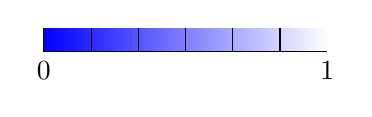
\begin{tikzpicture}[scale=0.6]
    \fill[left color=blue, right color=white] (0,0) rectangle (6,0.5);
    \draw (0,0) -- (6,0);
    \foreach \x in {0,20,...,100}
        \draw ({\x/20},0) -- ({\x/20},0.5);
    \node[below] at (0,0) {\MinValue};
    \node[below] at (6,0) {\MaxValue};
\end{tikzpicture}
\end{table}


% PCA reconstructed Iself beta frequency %

\begin{table}[ht]
\centering
\caption{PCA reconstructed Iself beta frequency}
\vspace{10pt} % Add more space here
\begin{tabular}{c *{5}{R}}
\multicolumn{1}{c}{} & \multicolumn{1}{c}{Matched} & \multicolumn{1}{c}{One-Head} & \multicolumn{1}{c}{One-Data} & \multicolumn{1}{c}{Random} & \multicolumn{1}{c}{Sensor} \\
AECno ort & 0.9879 & 0.6844 & 0.9939 & 0.9888 & 0.8330\\
AECort & 0.9129 & 0.4890 & 0.9448 & 0.9152 & 0.6616\\
ciPLV &  0.9556 & 0.9520 & 0.9721 & 0.9517 & 0.9595\\
\end{tabular}

% Color Scale
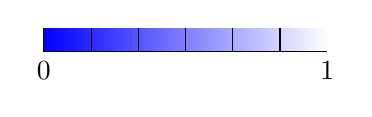
\begin{tikzpicture}[scale=0.6]
    \fill[left color=blue, right color=white] (0,0) rectangle (6,0.5);
    \draw (0,0) -- (6,0);
    \foreach \x in {0,20,...,100}
        \draw ({\x/20},0) -- ({\x/20},0.5);
    \node[below] at (0,0) {\MinValue};
    \node[below] at (6,0) {\MaxValue};
\end{tikzpicture}
\end{table}


% PCA reconstructed Iself gamma frequency %

\begin{table}[ht]
\centering
\caption{PCA reconstructed Iself gamma frequency}
\vspace{10pt} % Add more space here
\begin{tabular}{c *{5}{R}}
\multicolumn{1}{c}{} & \multicolumn{1}{c}{Matched} & \multicolumn{1}{c}{One-Head} & \multicolumn{1}{c}{One-Data} & \multicolumn{1}{c}{Random} & \multicolumn{1}{c}{Sensor} \\
AECno ort & 0.9886 & 0.5427 & 0.9958 & 0.9895 & 0.7640\\
AECort & 0.9187 & 0.5110 & 0.9787 & 0.9224 & 0.7243\\
ciPLV & 0.9516 & 0.9441 & 0.9958 & 0.9578 & 0.9582\\
\end{tabular}

% Color Scale
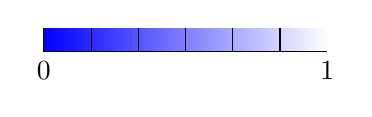
\begin{tikzpicture}[scale=0.6]
    \fill[left color=blue, right color=white] (0,0) rectangle (6,0.5);
    \draw (0,0) -- (6,0);
    \foreach \x in {0,20,...,100}
        \draw ({\x/20},0) -- ({\x/20},0.5);
    \node[below] at (0,0) {\MinValue};
    \node[below] at (6,0) {\MaxValue};
\end{tikzpicture}
\end{table}

% NON PCA reconstructed Iself Time Domain %

\begin{table}[ht]
\centering
\caption{NON PCA reconstructed Iself Time Domain}
\vspace{10pt} % Add more space here
\begin{tabular}{c *{5}{R}}
\multicolumn{1}{c}{} & \multicolumn{1}{c}{Matched} & \multicolumn{1}{c}{One-Head} & \multicolumn{1}{c}{One-Data} & \multicolumn{1}{c}{Random} & \multicolumn{1}{c}{Sensor} \\
Pearson's & 0.9754 & 0.9745 & 0.9870 & 0.9743 & 0.9417\\
\end{tabular}

% Color Scale
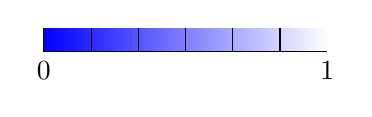
\begin{tikzpicture}[scale=0.6]
    \fill[left color=blue, right color=white] (0,0) rectangle (6,0.5);
    \draw (0,0) -- (6,0);
    \foreach \x in {0,20,...,100}
        \draw ({\x/20},0) -- ({\x/20},0.5);
    \node[below] at (0,0) {\MinValue};
    \node[below] at (6,0) {\MaxValue};
\end{tikzpicture}
\end{table}

% NON PCA reconstructed Iself delta frequency %

\begin{table}[ht]
\centering
\caption{NON PCA reconstructed Iself delta frequency}
\vspace{10pt} % Add more space here
\begin{tabular}{c *{5}{R}}
\multicolumn{1}{c}{} & \multicolumn{1}{c}{Matched} & \multicolumn{1}{c}{One-Head} & \multicolumn{1}{c}{One-Data} & \multicolumn{1}{c}{Random} & \multicolumn{1}{c}{Sensor} \\
AECno ort & 0.9497 & 0.9504 & 0.9579 & 0.9507 & 0.6114\\
AECort &  0.6746 & 0.6674 & 0.5758 & 0.6739 & 0.4248\\
ciPLV &  0.9491 & 0.9110 & 0.9202 & 0.9478 & 0.7222\\
\end{tabular}

% Color Scale
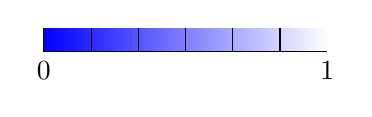
\begin{tikzpicture}[scale=0.6]
    \fill[left color=blue, right color=white] (0,0) rectangle (6,0.5);
    \draw (0,0) -- (6,0);
    \foreach \x in {0,20,...,100}
        \draw ({\x/20},0) -- ({\x/20},0.5);
    \node[below] at (0,0) {\MinValue};
    \node[below] at (6,0) {\MaxValue};
\end{tikzpicture}
\end{table}

% NON PCA reconstructed Iself theta frequency %

\begin{table}[ht]
\centering
\caption{NON PCA reconstructed Iself theta frequency}
\vspace{10pt} % Add more space here
\begin{tabular}{c *{5}{R}}
\multicolumn{1}{c}{} & \multicolumn{1}{c}{Matched} & \multicolumn{1}{c}{One-Head} & \multicolumn{1}{c}{One-Data} & \multicolumn{1}{c}{Random} & \multicolumn{1}{c}{Sensor} \\
AECno ort & 0.9578 & 0.9571 & 0.9771 & 0.9572 & 0.7009\\
AECort & 0.7349 & 0.7219 & 0.7642 & 0.7420 & 0.4987\\
ciPLV & 0.9539 & 0.9267 & 0.9366 & 0.9537 & 0.7665\\
\end{tabular}

% Color Scale
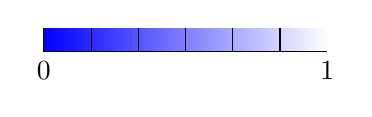
\begin{tikzpicture}[scale=0.6]
    \fill[left color=blue, right color=white] (0,0) rectangle (6,0.5);
    \draw (0,0) -- (6,0);
    \foreach \x in {0,20,...,100}
        \draw ({\x/20},0) -- ({\x/20},0.5);
    \node[below] at (0,0) {\MinValue};
    \node[below] at (6,0) {\MaxValue};
\end{tikzpicture}
\end{table}

% NON PCA reconstructed Iself alpha frequency %

\begin{table}[ht]
\centering
\caption{NON PCA reconstructed Iself alpha frequency}
\vspace{10pt} % Add more space here
\begin{tabular}{c *{5}{R}}
\multicolumn{1}{c}{} & \multicolumn{1}{c}{Matched} & \multicolumn{1}{c}{One-Head} & \multicolumn{1}{c}{One-Data} & \multicolumn{1}{c}{Random} & \multicolumn{1}{c}{Sensor} \\
AECno ort & 0.9619 & 0.9613 & 0.9687 & 0.9625 & 0.7396\\
AECort & 0.7581 & 0.7527 & 0.7675 & 0.7646 & 0.5190\\
ciPLV & 0.9555 & 0.9292 & 0.9503 & 0.9547 & 0.7753\\
\end{tabular}

% Color Scale
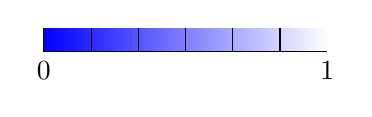
\begin{tikzpicture}[scale=0.6]
    \fill[left color=blue, right color=white] (0,0) rectangle (6,0.5);
    \draw (0,0) -- (6,0);
    \foreach \x in {0,20,...,100}
        \draw ({\x/20},0) -- ({\x/20},0.5);
    \node[below] at (0,0) {\MinValue};
    \node[below] at (6,0) {\MaxValue};
\end{tikzpicture}
\end{table}


% NON PCA reconstructed Iself beta frequency %

\begin{table}[ht]
\centering
\caption{NON PCA reconstructed Iself beta frequency}
\vspace{10pt} % Add more space here
\begin{tabular}{c *{5}{R}}
\multicolumn{1}{c}{} & \multicolumn{1}{c}{Matched} & \multicolumn{1}{c}{One-Head} & \multicolumn{1}{c}{One-Data} & \multicolumn{1}{c}{Random} & \multicolumn{1}{c}{Sensor} \\
AECno ort & 0.9819 & 0.9801 & 0.9859 & 0.9820 & 0.8472\\
AECort & 0.8425 & 0.8255 & 0.8153 & 0.8351 & 0.7110\\
ciPLV & 0.9839 & 0.9741 & 0.9821 & 0.9841 & 0.9041\\
\end{tabular}

% Color Scale
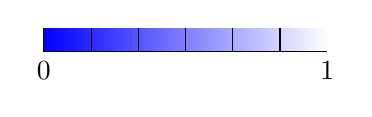
\begin{tikzpicture}[scale=0.6]
    \fill[left color=blue, right color=white] (0,0) rectangle (6,0.5);
    \draw (0,0) -- (6,0);
    \foreach \x in {0,20,...,100}
        \draw ({\x/20},0) -- ({\x/20},0.5);
    \node[below] at (0,0) {\MinValue};
    \node[below] at (6,0) {\MaxValue};
\end{tikzpicture}
\end{table}


% NON PCA reconstructed Iself gamma frequency %

\begin{table}[ht]
\centering
\caption{NON PCA reconstructed Iself gamma frequency}
\vspace{10pt} % Add more space here
\begin{tabular}{c *{5}{R}}
\multicolumn{1}{c}{} & \multicolumn{1}{c}{Matched} & \multicolumn{1}{c}{One-Head} & \multicolumn{1}{c}{One-Data} & \multicolumn{1}{c}{Random} & \multicolumn{1}{c}{Sensor} \\
AECno ort & 0.9787 & 0.9767 & 0.9902 & 0.9791 & 0.8208\\
AECort & 0.8733 & 0.8548 & 0.9186 & 0.8759 & 0.7716\\
ciPLV &  0.9828 & 0.9732 & 0.9939 & 0.9831 & 0.8942\\
\end{tabular}

% Color Scale
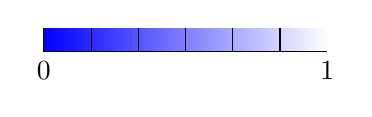
\begin{tikzpicture}[scale=0.6]
    \fill[left color=blue, right color=white] (0,0) rectangle (6,0.5);
    \draw (0,0) -- (6,0);
    \foreach \x in {0,20,...,100}
        \draw ({\x/20},0) -- ({\x/20},0.5);
    \node[below] at (0,0) {\MinValue};
    \node[below] at (6,0) {\MaxValue};
\end{tikzpicture}
\end{table}
\end{document}
